\pagestyle{MyStyle}

\begin{refsection}

\chapter{Summary and general discussion}
\label{ch:summary}

\newpage

\noindent
In this chapter, I will first summarize the main findings presented in this thesis, followed by a general discussion with a comprehensive literature review. The discussion is categorized into two parts: 1) multiscale wiring principles of the human brain connectome, and 2) multiscale neuropathology of schizophrenia. Furthermore, methodological considerations of the present thesis and future directions in the field of multiscale neuroscience will be deliberated. 

\section*{Summary}
Integrating the genetic, histological, and brain imaging data have provided a rich body of evidence for the relationship across multiscale brain organization \citep{Heuvel2019MultiscaleNO,Scholtens2018MultimodalCI}. Studies on non-human mammalian species have shown that the similarity of the microscale cortical cytoarchitecture is associated with the formation of macroscale cortico-cortical connectivity \citep{barbas2015general,beul2015predictive,beul2017predictive}. \textbf{Chapter 2} investigates whether such a micro-macro association is evolutionarily conserved in the human brain, by combining the state-of-the-art ultra-high-resolution BigBrain dataset and the macroscale human brain connectome. BigBrain data, which delineate the microscale cytoarchitecture, such as cell density and cell size \citep{amunts2013bigbrain}, were used in this study to capture the laminar cytoarchitectonic profile of human cortical regions. In parallel, the macroscale human connectome was reconstructed using diffusion weighted imaging (DWI) data of healthy individuals from the Human Connectome Project (HCP) \citep{VANESSEN201362}. Bridging the two ends of scales showed that the cytoarchitectonic profiles were more similar between interconnected cortical regions as compared to non-connected regions. The level of the cytoarchitectonic profile similarity was positively correlated with the connectivity strength, suggesting that cortical regions with more similar cytoarchitecture tend to be stronger connected by white matter connections. These results thus confirm one of the important wiring principles of the connectome – the microscale cortical cytoarchitectonic similarity shapes the macroscale brain connectome organization – to be evolutionarily conserved in the human brain. 


The relationship of microscale cytoarchitecture and macroscale connectivity reflects the commonality across species, now the question arises as to how the human connectome is differentiated from other non-human primates to support human’s complex cognitive abilities. Thus, in \textbf{Chapter 3}, I demonstrate the wiring principles of higher-order cognitive networks from the perspective of evolutionary genetics. In the human brain, there are functional networks, such as the frontoparietal network (FPN), salience network (SN), and default-mode network (DMN), supporting higher-order brain functions that differentiate human from other intelligent evolutionary relatives \citep{buckner2013evolution}. I thus hypothesized that brain regions of these higher-order cognitive networks are largely expanded in human evolution and this expansion is influenced by the underlying genetic differences between humans and other non-human primates. To test this hypothesis, cortical ribbon of humans and chimpanzees was first reconstructed using magnetic resonance imaging (MRI) data, and surface area of homologous cortical regions was compared between humans and chimpanzees. This comparison showed the highest cortical expansion in regions of higher-order cognitive networks, such as the FPN and DMN, in the human brain. Next, the pattern of brain expansion was linked to the gene expression pattern of the human-accelerated genes (HAR genes) in the human brain. Brain regions with more expansion in human evolution were found to demonstrate higher expression levels of HAR genes, with regions of the DMN showing the highest level of HAR gene expression. Comparative gene expression analysis further showed that HAR genes were differentially more expressed in higher-order cognitive networks in humans compared to chimpanzees and macaques. These findings together suggest that the upregulated expression of HAR genes may have played a role in the large expansion of cognitive functional networks during human brain evolution. Furthermore, \textbf{Chapter 3} identified a set of genes with specifically over-expression in the DMN and noted this gene set to be significantly overrepresented in HAR genes, and to be involved in synapse and dendrite formation. HAR genes and DMN-related genes show significant associations with individual variations in high-order cognitive functions, namely intelligence and sociability, and with risks of mental conditions, such as schizophrenia and autism. These findings highlight the potential role of HAR genes in shaping the higher-order cognitive functional networks in the human brain, and ultimately influencing cognitions and behaviors, and resulting in mental disorders of humans.

Examining the transcription-neuroimaging association provides insights for functional annotation of genes of interests and for exploration of genes associated with specific phenotypes of cognitive abilities or brain disorders. In \textbf{Chapter 4}, I present an integrative online platform, GAMBA (short for Gene Annotation using Macroscale Brain-imaging Association), which can be used to easily scrutinize the potential gene-transcription-neuroimaging associations. Given a set of genes of interest, GAMBA displays the cortical expression profile of these genes derived from the Allen Human Brain Atlas (AHBA) dataset \citep{Hawrylycz2012AnAC} and its associations to spatial patterns of a wide range of neuroimaging phenotypes, including the topological layout of resting-state brain functional networks, brain structural connectivity, cognitive components, cortical metabolic properties, functional and structural alterations across a range of brain disorders, et cetera. As an example of the application of GAMBA, I presented the cortical transcriptional profile of genes involved in microscale neuronal connectivity and its association with the organization of macroscale connectome. Moreover, I presented two examples in the context of brain disorders. One example showed APOE expression pattern to be associated with the pattern of brain structural/functional alterations in Alzheimer’s disease, and the other showed the association between expression of autism spectrum disorder (ASD) risk genes and brain functional alterations in Asperger’s syndrome. Together, GAMBA provides a user-friendly, open-source platform for functional annotation of genes with respect to macroscale neuroimaging-derived phenotypes of the healthy and diseased brain.

Schizophrenia is a mental disorder that is characterized by brain disconnectivity, in particular disconnectivity among highly connected rich-club regions \citep{vanDenHeuvel2013AbnormalRC}. However, confounded by factors such as prior therapeutic exposure and the potential influence of chronicity, it remained unclear to what extent the rich-club disconnectivity reflects the pathophysiology inherent to the nature of schizophrenia. \textbf{Chapter 5} thus aimed to examine the connectome abnormalities in first-episode, medication-naïve schizophrenia patients whose medical therapy is absent. To do so, DWI data and resting-state fMRI data from two independent samples were collected, including a principal dataset of 42 medication-naïve, previously untreated patients and 48 healthy controls, and a replication dataset of 39 first-episode patients (10 untreated patients) and 66 healthy controls. The connectome was reconstructed and the rich club organization was analyzed and compared between patients and controls. I showed that the rich club organization was significantly disrupted in medication-naïve schizophrenia patients as compared to healthy controls, with decreased rich-club connection strength in patients. The coupling between structural connectivity and functional connectivity among rich club regions was also decreased in medication-naïve schizophrenia patients. Using the replication dataset revealed similar results. These findings suggest that the disruption of rich club organization and functional dynamics may reflect an early feature of schizophrenia pathophysiology, which is independent of therapeutic exposure.

Observations of the association between microscale cytoarchitecture and macro-scale connectome in the human brain lead to the assumption that macroscale brain disconnectivity in schizophrenia could be related to microscale neuropathology \citep{Heuvel2019MultiscaleNO}. \textbf{Chapter 6} offers novel evidence for this cross-scale association by using in vivo magnetization transfer imaging (MTI), which describes an indirect measurement of brain microstructure, such as myelination \citep{Whitaker2016AdolescenceIA}. MTI data and DWI data from 78 schizophrenia patients and 93 healthy controls were collected to compute the magnetization transfer ratio (MTR) and to reconstruct the brain connectome, respectively. Significant MTR reductions were observed in prefrontal cortical regions, including bilateral rostral middle frontal areas, and right pars orbitalis and frontal pole, in schizophrenia patients as compared to controls. This finding confirms the prefrontal disruption of brain microstructure \citep{Garey1998ReducedDS, Glantz2000DecreasedDS}. Moreover, the cortical pattern of MTR reduction was observed to be associated with the pattern of macroscale dysconnectivity in schizophrenia, implicating regions with more myelination reduction to have more connectivity disruptions at the macroscale. This study thus provides empirical evidence for the prefrontal neuropathology in schizophrenia and further suggests the microscale deficits be associated with macroscale connectome abnormalities in schizophrenia.


\section*{General discussion}
\subsection*{Multiscale wiring principles of the human brain connectome}
The major goal of this thesis is to provide new insights into the wiring principles of the human brain connectome, namely, the rules governing the formation of macroscale structural and functional brain connectivity. Emerging evidence across a wide range of species has identified two evolutionarily conserved topological principles of the connectome: the community structure and the hub/rich-club organization \citep{Heuvel2016ComparativeC}. The community structure at the macroscale describes that spatially or functionally close brain regions are preferentially connected to each other to form distinct communities that are functionally specialized in certain cognitive domains \citep{smith2009correspondence,Sporns2016ModularBN,Wei2017IdentifyingTM}. These distributed communities are connected by hub/rich-club brain regions via long-range and costly connections to enable efficient neural information integration within the whole brain \citep{vanDenHeuvel2012HighcostHB,Senden2014RichCO}. Therefore, the hub/rich-club organization displays a trade-off between minimizing the cost of neural resources and maximizing the efficiency of information communication \citep{bullmore_economy_2012,Heuvel2019ACC}. This thesis discusses and extends these two topological motifs in the context of the microscale brain structure to gain a deeper understanding of the biological wiring principles of the human brain connectome.

Results in \textbf{Chapter 2} support the notion that the microscale cytoarchitecture of cortical regions plays a role in shaping the macroscale brain connectivity. Neuroanatomical studies have demonstrated varied cytoarchitectonic features across the cortex, such as the number and thickness of cortical layers, degree of visibility of layer IV, cell packing density, etc. \citep{brodmann1909vergleichende, von1925cytoarchitektonik,Uluda2015fMRIFN}. These cytoarchitectonic features are claimed to follow a system-level gradient from the primary sensory/motor to the association and eventually to the limbic system \citep{Uluda2015fMRIFN,Paquola2019MicrostructuralAF}. Studies combining microscale cytoarchitectonic information and macroscale anatomical connectivity have indicated that the cytoarchitectonic similarity between brain regions could predict the existence of their interconnections at the macroscale \citep{barbas2015general,GarcaCabezas2019TheSM}. This hypothesis, known as "structural model”, evidenced as brain regions with more similar cytoarchitecture are more likely to be connected by white matter fibers in a wide range of species, such as mouse \citep{goulas2017principles}, cat \citep{beul2015predictive}, and macaque \citep{Hilgetag2010CytoarchitecturalDA,beul2017predictive}. Our observation of the associated cytoarchitectonic profile similarity and cortico-cortical connectivity in the human brain in \textbf{Chapter 2} suggests the "structural model” to be evolutionarily conserved in the human brain \citep{WEI2019bigbrain}. Furthermore, such an association between cytoarchitecture and anatomical connectivity aligns with the findings of the functional connectome. The macroscale functional network architecture has been shown to be associated with the similarity of cytoarchitecture and myeloarchitecture in the human brain \citep{Paquola2019MicrostructuralAF,Hunt2016RelationshipsBC,Huntenburg2017ASR}, indicating \textbf{the similarity of cellular-level brain structure as a underlying neural basis for the formation of structural and functional networks in the human brain}.

This kind of "similar-prefer-similar" principle of the connectome organization may be explained in several aspects. First, the shared developmental trajectory of the brain cytoarchitecture and brain connectivity may determine the association between microscale cytoarchitectonic similarity and macroscale brain connectivity. Briefly, brain regions with similar cytoarchitecture are likely to develop within a similar time window that overlaps in the course of brain connectivity formation \citep{barbas2015general,hilgetag2016primate,beul2017predictive}. Moreover, the associated cytoarchitectonic similarity and macroscale connectivity may be driven by the shared transcriptional signatures between two brain regions. Genetic findings have shown that brain regions with more similar gene expression profiles are preferentially connected by macroscale white matter connections \citep{French2011RelationshipsBG}. The highest similarity of gene expression profiles corresponds to connections between rich-club brain regions, with the second-highest similarity for connections between rich-club and non-rich-club regions, and the lowest similarity for connections between non-rich-club regions \citep{Fulcher2016ATS}. The coupled transcriptional profiles of genes also recapitulate patterns of resting-state brain functional networks \citep{richiardi2015correlated}. Specifically examining a subset of genes enriched in the supragranular layers of the human cortex has shown that brain regions with similar transcription profiles of these genes are tightly connected at the macroscale both structurally \citep{RomeroGarcia2018StructuralCN} and functionally \citep{krienen2016transcriptional}. As the supragranular layers of the cortex are known to be important for forming microscale cortico-cortical neuronal projections \citep{Zilles2015CytoarchitectureAM}, the above findings point to a cross-scale association among the transcriptional similarity, cytoarchitectonic similarity, and macroscale brain connectivity.

The association between the microscale brain structure and the macroscale connectome is further supported by \textbf{Chapter 3\&4}, which shows that human-accelerated genes (HAR genes) are over-expressed in brain regions of a range of higher-order cognitive networks. HAR genes are known to function as neuronal enhancers and play a pivotal role in neurogenesis \citep{Ryu256313}. Up-regulated expression of HAR genes in regions of cognitive functional networks thus may enable these brain regions with more complex neuronal structures \citep{elston2003cortex}. The more complex neuronal structure, such as higher dendritic spine density of layer III pyramidal neurons, has been linked to more white matter connections at the macroscale \citep{scholtens2014linking,VANDENHEUVEL2016293}. Therefore, this again points to a linkage across the microscale molecular and cellular structure, and the macroscale brain connectivity. This cross-scale linkage is also supported by findings showing that genes related to the functional connectivity of the DMN are those more expressed in neurons \citep{wang2015correspondence} and are involved in the formation of neuronal projections \citep{Wei2019GeneticMA}. Genes over-expressed in brain regions involved in long-range inter-module functional connectivity are also significantly enriched in the supragranular layers of the human cortex \citep{vertes2016gene}. Furthermore, as HAR genes correspond to genome regions conserved in other primates but strikingly differentiated in human, results in \textbf{Chapter 3} suggests \textbf{an evolutionary drive for the observed cross-scale association between neuronal complexity and functional networks that are important for human higher-order cognition}.

\textbf{Chapter 3} shows that the organization of the human brain functional network undergoes selection pressure during human evolution. Despite that humans and non-human primates share a similar pattern of functional network, such as the DMN \citep{mantini2011default,barks2013default}, association brain regions involved in the DMN and other higher-order cognitive networks have been largely expanded in the human brain compared to the brain of non-human primates \citep{hill2010similar,donahue2018quantitative}. White matter connections linking these frontal and temporal association areas in the human brain also overrepresent with connections that are uniquely observed in humans but not in chimpanzees \citep{ardesch2019evolutionary}. Such differentiations presented in association areas at the macroscale are associated with an over-expression of evolutionarily important genes, namely HAR genes in the human genome (\textbf{Chapter 3}). It implies that \textbf{the evolutionary differentiation of the macroscale brain connectivity is driven by the differentiation of the genome}. Moreover, these evolutionary differences at the two ends of the scale may also relate to a much longer period of neuronal progenitor expansion observed in humans compared to chimpanzees and macaques \citep{otani20162d}. The differentiated neuronal progenitor expansion may result in a more complex neuronal structure in association regions \citep{elston2001pyramidal} and ultimately higher computational capacity to support complicated cognitive abilities of humans \citep{Bianchi2013DendriticMO,Goriounova2018LargeAF,reardon2018normative}. However, these evolutionary changes may also make higher-order cognitive networks more vulnerable to psychiatric conditions \citep{Wei2019GeneticMA}, in particular, schizophrenia \citep{Heuvel2019EvolutionaryMI}.

\subsection*{Multiscale neuropathology in schizophrenia}
Schizophrenia has long been suggested as a disorder of brain disconnectivity \citep{Stephan2009DysconnectionIS,Fitzsimmons2013ReviewOF}. While disruptions of structural connectivity in schizophrenia are widespread across the entire brain, the disconnectivity pattern topologically converges to brain hub/rich-club regions \citep{Klauser2017WhiteMD}. Connections between hub/rich-club regions consistently show reductions in the connectivity strength in schizophrenia \citep{vanDenHeuvel2013AbnormalRC,Griffa2015CharacterizingTC,Klauser2017WhiteMD}. Such reductions have also been revealed in first-episode, medication-naïve schizophrenia patients in \textbf{Chapter 5} \citep{CUI2019SCZ}, suggesting \textbf{rich club abnormality in schizophrenia as a white matter pathology regardless of the drug usage}. Complementing this finding, rich club disruptions have been found in unaffected siblings \citep{Collin2014ImpairedRC} and young offspring of schizophrenia patients \citep{Collin2017AffectedAR}, further suggesting the potential genetic substrates underlying the disconnectivity pattern in schizophrenia.

The genome-wide association studies (GWAS) in schizophrenia have revealed a complex genetic component of schizophrenia \citep{Ripke2014BiologicalIF,Li2017GenomewideAA}. Multiple genomic loci, for example loci in \textit{DRD2} and several genes involved in glutamatergic neurotransmission, together contribute to the etiology of schizophrenia \citep{Ripke2014BiologicalIF}. Cross-scale examinations have further shown that genetic risks of schizophrenia are associated with macroscale brain structure and function. Specifically, polygenic risks of schizophrenia have been observed to be associated with individual variability in gray matter and white matter volume \citep{Scheltinga2013GeneticSR}, cortical thickness \citep{Alns2019BrainHI}, structural connectivity \citep{Alloza2018PolygenicRS}, functional connectivity \citep{Wang2017PolygenicRF}, and brain activity when processing working memory tasks \citep{Kauppi2015PolygenicRF}. Moreover, examining gene expression profiles of schizophrenia risk genes shows that brain regions with an over-expression of schizophrenia risk genes are more disconnected at the macroscale in schizophrenia \citep{Romme2017ConnectomeDA}. These findings further suggest that \textbf{brain processes at multiple scales are not independent and schizophrenia-related brain connectivity alterations at the macroscale are related to molecular changes at the microscale}.

Extended evidence for the cross-scale pathological association in schizophrenia came from studies examining the disease-related cellular abnormalities. Investigating cytoarchitecture alone has demonstrated a reduced dendritic spine density \citep{Garey1998ReducedDS,Glantz2000DecreasedDS,Kolluri2005LaminaspecificRI} and soma size \citep{Pierri2001DecreasedSS} of layer III pyramidal neurons in the prefrontal cortex in schizophrenia patients. Further, myeloarchitectonic studies have shown reduced density of oligodendrocytes, which are responsible for forming the myelin sheath around axons, in prefrontal regions in schizophrenia \citep{Uranova2011UltrastructuralAO,Uranova2004OligodendroglialDI}. The above microscale changes are very likely to be related to the macroscale brain alterations in schizophrenia, inferred by a strong correlation between the alteration of dendritic spine density of layer III pyramidal neurons and the macroscale white matter connectivity changes in schizophrenia \citep{VANDENHEUVEL2016293}. Moreover, the disruptions in cortical myelination, as discussed in \textbf{Chapter 6} \citep{Wei2018CorticalMT}, have also been suggested to be related to white matter connectivity changes in schizophrenia \citep{Cassoli2015DisturbedMI}. Taken together, \textbf{linking multiscale brain features in schizophrenia offers a more comprehensive understanding of the cross-scale pathway of schizophrenia, which is important for understanding the etiology of the disease}.

\begin{figure}[h]
    \centering
    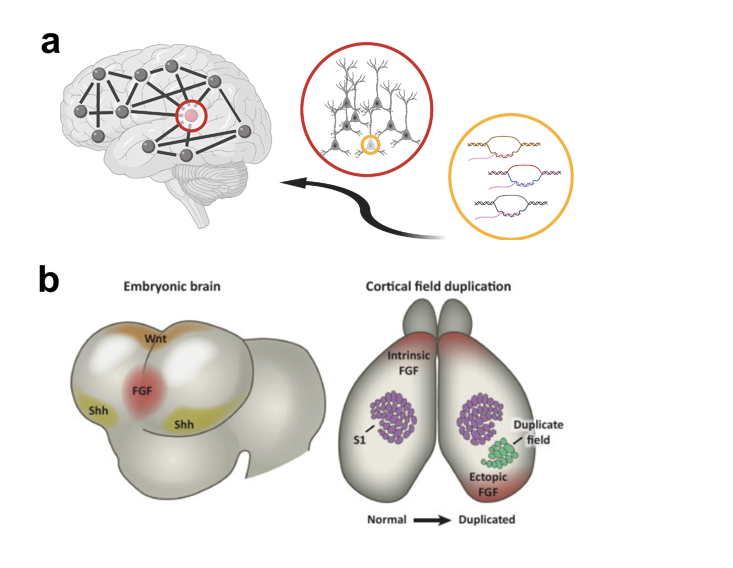
\includegraphics[width=10cm]{images/discussionFigure.png}
    \caption{Examples of mechanisms underlying multiscale neuroscience. (a) The proposed mechanism of a step-by-step accumulation from gene transcription (yellow circle) to neuronal structure (red circle) and then to macroscale connectome organization. Created with BioRender.com. (b) The proposed molecular constraints on cortical formation. Left: molecular gradient of Wnt (orange), fibroblast growth factor (FGF) (red), and sonic hedgehog (Shh) (yellow) are expressed at specific locations in the telencephalon of the mouse embryo. Right: Manipulating signaling molecules changes cortical structures. As presented in \citep{FukuchiShimogori2001NeocortexPB}, expressions of FGF8 in the posterior telencephalon can lead to duplicated S1 area. Reprinted from "The evolution of distributed association networks in the human brain", by Authors R.L. Buckner et al., 2013, Trends in Cognitive Sciences, 17(12), 648-665. Copyright [2013] by Elsevier. Reprinted with permission.}
    \label{disFig4}
\end{figure}

\subsection*{The principle of multiscale neuroscience}
The current thesis suggests that the macroscale connectome organization is associated with the microscale genetic and cellular features, pointing to the principle of multiscale neuroscience of the healthy and diseased brain \citep{Heuvel2019MultiscaleNO}. One proposed mechanism underlying multiscale neuroscience is a step-by-step accumulation from genes to proteins, cells, neuronal circuits, and ultimately macroscale brain organization (see Figure \ref{disFig4}a). This mechanism also suggests that genotypic variants for risks in brain disorders may bring disruptions in protein and neuron structure, which are piled up to brain abnormalities revealed at the macroscale. Apart from the accumulation of brain "building blocks", another potential mechanism underlying multiscale neuroscience suggests that microscale brain attributes may exert constraints on the formation of macroscale brain structural and functional organization. The structural model \citep{GarcaCabezas2019TheSM} is a good example for such constraints. The topology of the systematic variation of the cortex forms constraints across different scales, with brain regions sharing similar transcriptional profiles and structural types to have a higher chance of being structurally and functionally connected. Another example of the cross-scale constraints is the tethering hypothesis stating the formation of distributed cognitive networks at the macroscale \citep{buckner2013evolution} (Figure \ref{disFig4}b). This hypothesis assumes that there are a handful of anchors, including V1, S1, A1, and the MT area, emerge early during the development of the human brain from constraints of molecular gradients \citep{Rakic2009EvolutionOT} and typical thalamocortical inputs \citep{OLeary2008GeneticRO}. Spatial gaps between these anchors are further dominated by self-organizing activity-dependent interactions to form the prefrontal, temporal, and parietal association cortices. In parallel to the above-mentioned mechanisms of the step-by-step accumulation and the cross-scale constraints, an alternative mechanism underlying multiscale neuroscience suggests that the macroscale brain organization provides a guidance for activities at the microscale. For example, the organization of macroscale brain functional networks has been proposed to be able to regulate the spread of cellular pathology in neurological disorders \citep{Buckner2009CorticalHR,Seeley2009NeurodegenerativeDT,Zhou2012PredictingRN}. It is noteworthy that all these possible mechanisms of multiscale neuroscience may not be independent, but also interact with each other to form complex neural systems that support humans’ cognitive abilities and behaviors. 


\subsection*{Methodology considerations and future directions}
Several methodological considerations need to be remarked when interpreting results in this thesis. Many of these considerations also point to opportunities for future studies. 

\subsubsection*{Individual variation}
Studies in \textbf{Chapter 2} and \textbf{3} bridge the microscale transcriptomics and cytoarchitecture and to the macroscale brain connectome based on data resources acquired across different individuals, such as the BigBrain data \citep{amunts2013bigbrain}, Allen Human Brain Atlas \citep{Hawrylycz2012AnAC}, psychENCODE dataset \citep{sousa2017molecular}, and MRI data from the Human Connectome Project \citep{VANESSEN201362}. The cross-scale association is mainly built upon the relationship of group-level spatial profiles across brain regions rather than across individuals, such that the individual variation of multiscale features of the human brain is inherently overlooked. Studying individual variation is quite challenging until now as it requires different scales of data from the same subjects. Therefore, new dataset delineating multiscale brain structure and function from the same subjects would be of great value. Psychiatric brain banks \citep{DeepSoboslay2011PsychiatricBB} that collect multiscale data from brain tissues of psychiatric patients may allow connecting individual variations across different scales. Moreover, the advance of image technology and analytic methods provides promising approaches to assess microscale brain structure. For example, the contrast of T1- and T2-weighted MRI \citep{Glasser2011MappingHC} and MTR imaging (\textbf{Chapter 5}) have been widely used to measure the extent of cortical myelination \citep{Heath2018AdvancesIN}. Ultra-high-field quantitative MRI has the potential to assess the in vivo laminar structure \citep{Trampel2017InvivoMR} and molecular composition \citep{Filo2019DisentanglingMA} of the human cortex. These developments in imaging techniques may make it feasible to obtain in vivo multiscale information from larger samples of human subjects and to bridge individual variations of microscale cytoarchitecture and myeloarchitecture and macroscale connectome.

\subsubsection*{Sample size}
An additional consideration is the relatively small sample size of some of the examined datasets in this thesis due to the highly complex and expensive processes in data acquisition. The small sample size makes it challenging for validation and generalization of the results. In this thesis, we put large efforts into validation. For example, we used the Von Economo - Koskinas atlas to show the validity of BigBrain profiles examined in \textbf{Chapter 2} and replicated the major findings in \textbf{Chapter 3} by using both the AHBA dataset and psychENCODE dataset. However, future studies increasing the data sample size to allow validations based on separate sets of samples with similar configurations, as similar to what \textbf{Chapter 4} does, would still be of great importance to generalize the discussed multiscale associations.  

\subsubsection*{Causality}
It should be noted that the cross-reference of multiscale brain features showed in \textbf{Chapter 2, 3, 6} could not provide information about the causal interactions, which are important for understanding the biological mechanism underlying the observed associations. To gain a better insights of the causality of the observed cross-scale associations, future studies making modifications at one scale and then examining alterations at the other scale would be of great help. For instance, gene-editing CRISPR technique opens up a new avenue for the inference of causality \citep{Doudna2014TheNF}, with promising findings showing that \textit{APOE4} variant, which relates to risks in Alzheimer’s disease, causes gene expression differentiations for genes specifically involved in synaptic function \citep{Lin2018APOE4CW}. In addition, longitudinal studies enabling to examine the developmental trajectory of multiscale changes and the course of diseases should be considered to provide information about the time-lag-based causality across scales.

\subsection*{Conclusions}
This thesis investigates the association between the macroscale brain connectome organization and the microscale cortical cytoarchitecture and gene transcription. It also provides evidence for the macroscale disconnectivity in schizophrenia and its relationship to the microscale neuropathology of the disease. Binding genes, neurons, and the connectome, this thesis offers novel insights into the neurobiological wiring principles of the human brain connectome and the disconnectivity pattern in schizophrenia. Integrating multiscale information on brain structure and function paves a new avenue to disentangle the complex neurobiological mechanisms of human cognition and brain disorders.

\printbibliography[heading=subbibliography]

\end{refsection}